%%%%%%%%%%%%%%%%%%%%%%%%%%%%%%%%%%%%%%%%%%%%%%%%%%%%%%%%%%%%%%%%%%%%%%%%%%%%%%%%%%%%%%%%%%%%%%%%%%%%%
% This template is distributed with ABSOLUTELY NO WARRANTY.
% It serves as a guideline and constitutes a basic structure for a
% thesis/dissertation. The user assumes full responsibility for formatting
% and typesetting their document and for verifying that all the thesis
% requirements set by the University of Tennessee are met. Please refer to the most
% recent UT thesis guide (http://gradschool.utk.edu/thesesdissertations/formatting/)
% or contact the thesis consultant (http://gradschool.utk.edu/thesesdissertations/).
% Please report any bugs to the thesis consultant.
%%%%%%%%%%%%%%%%%%%%%%%%%%%%%%%%%%%%%%%%%%%%%%%%%%%%%%%%%%%%%%%%%%%%%%%%%%%%%%%%%%%%%%%%%%%%%%%%%%%%%
% O P T I O N S:
% 1. thesis/dissertation
% 2. monochrome
% 3. all options provided by the report class
%%%%%%%%%%%%%%%%%%%%%%%%%%%%%%%%%%%%%%%%%%%%%%%%%%%%%%%%%%%%%%%%%%%%%%%%%%%%%%%%%%%%%%%%%%%%%%%%%%%%%
%First, is this a thesis or dissertation? Choose one by commenting out the one you don't need:
%\documentclass[thesis,letterpaper,12pt]{utthesis} % thesis
\documentclass[dissertation,letterpaper,12pt]{utthesis} %dissertation

% Algorithms
\usepackage[linesnumbered, lined, ruled, boxed]{algorithm2e}

%Table background color
\usepackage[table,xcdraw]{xcolor}

% some alternatives are:
%\documentclass[thesis,monochrome,letterpaper,12pt]{utthesis} %thesis, monochrome text
\renewcommand{\baselinestretch}{1.5} 	 % line Spacing

%%%%%%%%%%%%%%%%%%%%%%%%%%%%%%%%%%%%%%%%%%%%%%%%%%%%%%%%%%%%%%%%%%%%%%%%%%%%%%%%%%%%%%%%%%%%%%%%%%%%%
% TO DO: FILL IN YOUR INFORMATION BELOW - READ THIS SECTION CAREFULLY
%%%%%%%%%%%%%%%%%%%%%%%%%%%%%%%%%%%%%%%%%%%%%%%%%%%%%%%%%%%%%%%%%%%%%%%%%%%%%%%%%%%%%%%%%%%%%%%%%%%%%
\title{ Yout thesis Title ..............}

% title of thesis/dissertation
\author{ Your  full name  }                			% author's name
\copyrightYear{2021}            				% copyright year of your thesis/dissertation
\graduationMonth{December}           				% month of graduation for your thesis/dissertation
\degree{Doctor of Philosophy / master ? }	    			% degree: Doctor of Philosophy, Master of Science, Master of Engineering...
\university{University of Tennessee at Chattanooga}	% school name
%%%%%%%%%%%%%%%%%%%%%%%%%%%%%%%%%%%%%%%%%%%%%%%%%%%%%%%%%%%%%%%%%%%%%%%%%%%%%%%%%%%%%%%%%%%%%%%%%%%%%
% LOAD SOME USEFUL PACKAGES. 
% No need to change anything here, although if you'd like to add packages you can do that here. Note that packages preloaded with the utthesis class are: amsmath,amsthm,amssymb,setspace,geometry,hyperref,and color
%%%%%%%%%%%%%%%%%%%%%%%%%%%%%%%%%%%%%%%%%%%%%%%%%%%%%%%%%%%%%%%%%%%%%%%%%%%%%%%%%%%%%%%%%%%%%%%%%%%%%

\usepackage{tocloft} 
\usepackage{mathptmx}                   % for Times New Roman-like font
\usepackage{nomencl}                    % produces a nomenclature
\usepackage{float}                      % figure floats
\usepackage[numbers]{natbib}            % this package allows you to link your references
\usepackage{graphicx}					% graphics package

% figure path ......
\graphicspath{ {figures/}{figures/ieee/}{figures/plusone/}} 
\usepackage{fancyhdr}                   % fancy headers and footers
\usepackage{url}                        % nicely format url breaks
\usepackage[inactive]{srcltx}		 	% necessary to use forward and inverse searching in DVI
\usepackage{relsize}                    % font sizing hierarchy
\usepackage{booktabs}                   % professional looking tables
\usepackage[config]{caption,subfig} % nice sub figures
\usepackage{mathrsfs}                   % additional math scripts
\usepackage[page,toc,titletoc,title]{appendix}			% format appendix correctly
\usepackage{pdflscape}					% to produce landscape pages if necessary
% \usepackage{algorithm}                  % For pseudo code examples
\usepackage{algorithmic}                % For pseudo code examples

% Algorithms
\usepackage[linesnumbered, lined, ruled, boxed]{algorithm2e}

%Table background color
\usepackage[table,xcdraw]{xcolor}
%%%%%%%%%%%%%%%%%%%%%%%%%%%%%%%%%%%%%%%%%%%%%%%%%%%%%%%%%%%%%%%%%%%%%%%%%%%%%%%%%%%%%%%%%%%%%%%%%%%%%%
% Table of contents tinkering
%%%%%%%%%%%%%%%%%%%%%%%%%%%%%%%%%%%%%%%%%%%%%%%%%%%%%%%%%%%%%%%%%%%%%%%%%%%%%%%%%%%%%%%%%%%%%%%%%%%%%%
\renewcommand{\contentsname}{\hfill\normalfont\normalsize TABLE OF CONTENTS\hfill}   % Change table of contents heading font
\renewcommand{\cftaftertoctitle}{\hfill}        % Needed with the above code?
\setlength{\cftaftertoctitleskip}{2\baselineskip} % Adds only two lines after the heading

\renewcommand{\cftlottitlefont}{\hfill\normalfont\normalsize} % Changes List of Tables heading font
\renewcommand{\cftafterlottitle}{\hfill}
\setlength{\cftafterlottitleskip}{2\baselineskip}

\renewcommand{\cftloftitlefont}{\hfill\normalfont\normalsize} % Changes List of Figures heading font
\renewcommand{\cftafterloftitle}{\hfill}
\setlength{\cftafterloftitleskip}{2\baselineskip}

\setlength{\cftbeforechapskip}{\baselineskip}           % Add spacing after each chapter
\renewcommand{\cftchapleader}{\cftdotfill{\cftdotsep}}  % Add the dots to chapters in the TOC

\renewcommand\cftchapfont{\mdseries}            % No bold for chapter names
\renewcommand\cftchappagefont{\mdseries}        % No bold for chapter names
\renewcommand\cftchapaftersnum{.}               % Add dot after chapter number in TOC
\setcounter{tocdepth}{4}
\setcounter{secnumdepth}{4}
%%%%%%%%%%%%%%%%%%%%%%%%%%%%%%%%%%%%%%%%%%%%%%%%%%%%%%%%%%%%%%%%%%%%%%%%%%%%%%%%%%%%%%%%%%%%%%%%%%%%%%
% Chapter/Section tinkering
%%%%%%%%%%%%%%%%%%%%%%%%%%%%%%%%%%%%%%%%%%%%%%%%%%%%%%%%%%%%%%%%%%%%%%%%%%%%%%%%%%%%%%%%%%%%%%%%%%%%%%
\usepackage[indentafter]{titlesec}              % The package for adjusting chapter and sections
                                                % indentafter makes sure that all paragraphs have indents

\titleformat{\chapter}[display]                 % Adjust how the chapters look
  {\centering\normalfont\normalsize}
  {\MakeUppercase{\chaptertitlename}\ \thechapter}
  {.5em}
  {\MakeUppercase}

\titleformat*{\section}{\normalfont\normalsize}                     %Adjust the section headings
\titleformat*{\subsection}{\centering\normalfont\normalsize}%Adjust the subsection headings
\titleformat*{\subsubsection}{\centering\normalfont\normalsize\itshape}%Adjust the subsection headings

\titlespacing{\chapter}{0pt}{.7in}{*4}

% Adjust the spacing after each section!
% Here it is saying, no extra left tab (0pt), 2 times the current above spacing (so 2 lines)
% and 0 times the current spacing after the heading (so no extra lines).
\titlespacing{\section}{0pt}{*2}{*0} 
\titlespacing{\subsection}{0pt}{*2}{*0}
\titlespacing{\subsubsection}{0pt}{*2}{*0}

%%%%%%%%%%%%%%%%%%%%%%%%%%%%%%%%%%%%%%%%%%%%%%%%%%%%%%%%%%%%%%%%%%%%%%%%%%%%%%%%%%%%%%%%%%%%%%%%%%%%%%
% Figure/Table caption tinkering
%%%%%%%%%%%%%%%%%%%%%%%%%%%%%%%%%%%%%%%%%%%%%%%%%%%%%%%%%%%%%%%%%%%%%%%%%%%%%%%%%%%%%%%%%%%%%%%%%%%%%%
\captionsetup{format=hang}          % Add the hanging indent to table & figure captions
\captionsetup[table]{belowskip=12pt,aboveskip=\baselineskip,labelsep=space} % Adjust table properties
\captionsetup[figure]{aboveskip=24pt,labelsep=space}

\setlength{\cfttabindent}{0in}    %% Make LOT and LOF not use extra indent
\setlength{\cftfigindent}{0in}    %% Make LOT and LOF not use extra indent

% Derek 10-13-2020 from: https://groups.google.com/g/latexusersgroup/c/2IZlIK40dGA
% This code (and package) lets us make algorithm captions as figures
\usepackage{letltxmacro}
\LetLtxMacro{\oldalgorithmic}{\algorithmic}
\LetLtxMacro{\endoldalgorithmic}{\endalgorithmic}
\renewenvironment{algorithmic}[1][0]{%
  \hrulefill\par
  \oldalgorithmic[#1]}
  {\endoldalgorithmic\par
   \vspace*{-.5\baselineskip}
   \hrulefill\par
  }

%%%%%%%%%%%%%%%%%%%%%%%%%%%%%%%%%%%%%%%%%%%%%%%%%%%%%%%%%%%%%%%%%%%%%%%%%%%%%%%%%%%%%%%%%%%%%%%%%%%%%%
% This section formats landscape pages properly with the correct page number.
% This code is only necessary when landscape pages are needed and can be left alone
%%%%%%%%%%%%%%%%%%%%%%%%%%%%%%%%%%%%%%%%%%%%%%%%%%%%%%%%%%%%%%%%%%%%%%%%%%%%%%%%%%%%%%%%%%%%%%%%%%%%%%


\fancypagestyle{mylandscape}{
	\fancyhf{} %Clears the header/footer
	\fancyfoot{% Footer
    \makebox[\textwidth][r]{% Right
      \rlap{\hspace{.75cm}% Push out of margin by \footskip
        \smash{% Remove vertical height
          \raisebox{4.87in}{% Raise vertically
            \rotatebox{90}{\thepage}}}}}}% Rotate counter-clockwise
  \renewcommand{\headrulewidth}{0pt}% No header rule
  \renewcommand{\footrulewidth}{0pt}% No footer rule
}

%%%%%%%%%%%%%%%%%%%%%%%%%%%%%%%%%%%%%%%%%%%%%%%%%%%%%%%%%%%%%%%%%%%%%%%%%%%%%%%%%%%%%%%%%%%%%%%%%%%%%
\begin{document}
    \pagenumbering{alph} % this is needed to clear certain issues with the hyperref package
    %
    %\addToPDFBookmarks{0}{Front Matter}{rootNode} % create a root node named "Front Matter" in the pdf bookmarks
    \addToPDFBookmarks{1}{Title}{a} % add a pdf bookmark to the title page
    \makeCommitteePage  % make the committee page
    %
    \pagenumbering{roman}
    \setcounter{page}{2}
    %
    \makeTitlePage      % make the title page.
    %
    \makeCopyrightPage % make the copyright page
    %
%%%%%%%%%%%%%%%%%%%%%%%%%%%%%%%%%%%%%%%%%%%%%%%%%%%%%%%%%%%%%%%%%%%%%%%%%%%%%%%%%%%%%%%%%%%%%%%%%%%%%
%The dedication and acknowledgments are optional. If you wish not to include them, simply comment out both the "\addToPDF..." line and the "\include{...}" line for each.
%%%%%%%%%%%%%%%%%%%%%%%%%%%%%%%%%%%%%%%%%%%%%%%%%%%%%%%%%%%%%%%%%%%%%%%%%%%%%%%%%%%%%%%%%%%%%%%%%%%%%

    \makeAbstractPage
    \makeDedicationPage
    \makeAcknowlPage
   
    \addToPDFBookmarks{0}{TABLE OF CONTENTS}{f}
    \begin{spacing}{1}
    \tableofcontents % generate a table of contents
    \end{spacing}
    
    \makeListofTables % generate a list of tables
    \makeListofFigures % generate a list of figures
    \makeNomePage % generate list of nomenclature 
    %\makeAbbrPage % generate list of abbreviations
  
    % \makeAbbrPage

    \newpage
    \pagenumbering{arabic}
    \setcounter{page}{1}
    %%%%%%%%%%%%%%%%%%%%%%%%%%%%%%%%%%%%%%%%%%%%%%%%%%%%%%%%%%%%%%%%%%%%%%%%%%%%%%%%%%%%%%%%%%%%%%%%%%%%%
    % INCLUDE THE CHAPTERS STARTING WITH THE NOMENCLATURE IF PRESENT
    %%%%%%%%%%%%%%%%%%%%%%%%%%%%%%%%%%%%%%%%%%%%%%%%%%%%%%%%%%%%%%%%%%%%%%%%%%%%%%%%%%%%%%%%%%%%%%%%%%%%%
    \chapter{Introduction} 
\label{chapter:introduction}



%\begin{figure}[!h]
%\captionsetup{format=hang}
%\centering
%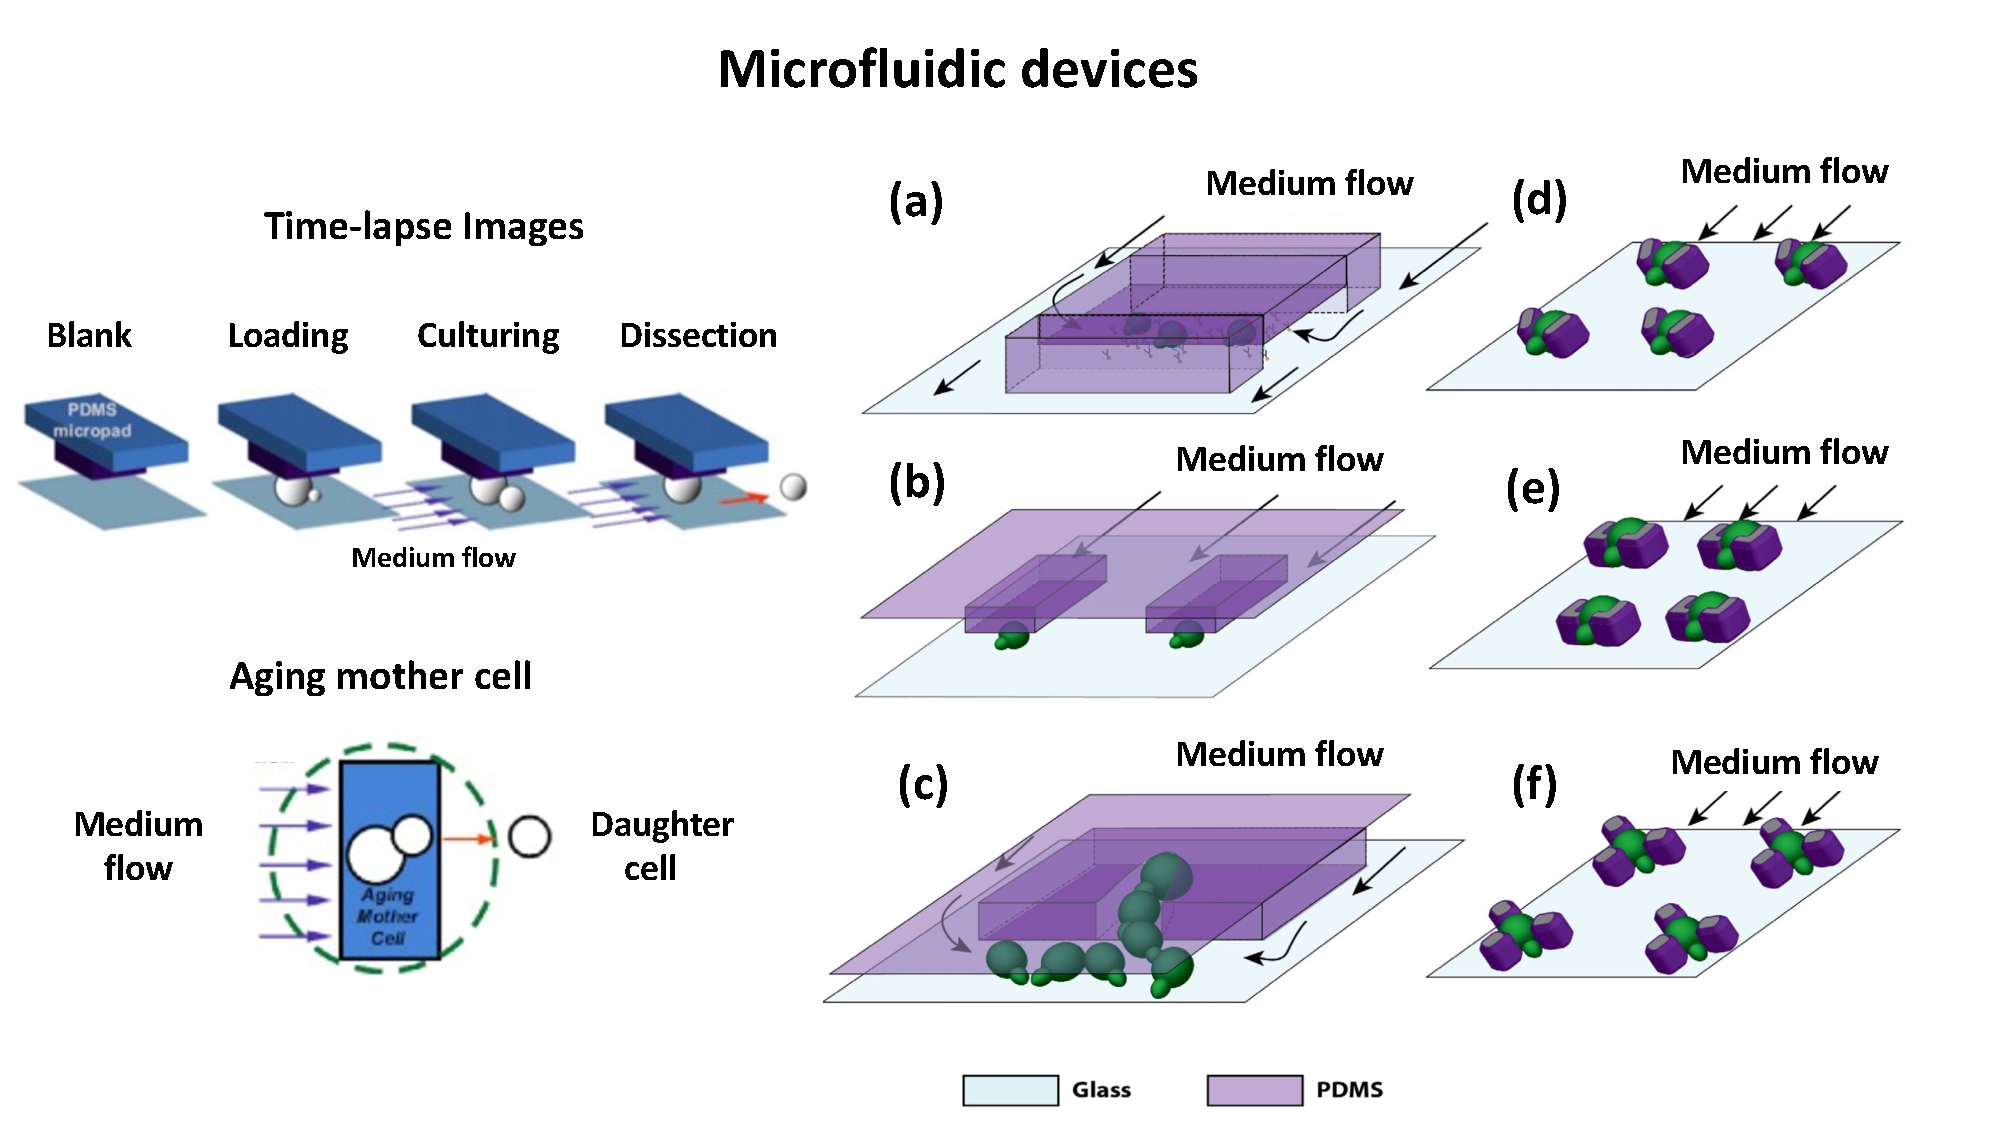
\includegraphics[width=1\textwidth,height=0.5\textheight,angle %=0]{dissertation/figures/data/microfludic.pdf}
%\caption{ The generic type of microfluidic devices. Patterns a, b and c %are considered as low-throughput. Patterns d, e, and f are considered as %high-throughput}
%\label{fig:micro}
%\end{figure} 


\section{Outline}

%The remainder of this dissertation is organized as follows. Chapter \ref{microfluidic} provides background and review of relevant literature surrounding segmentation methods and model comparison. Chapter \ref{classify} provides some information on microfluidic devices, time series microfluidic images and steps for data collection. Chapter \ref{Mask_yolo} covers deep learning model comparison for microfluidic image classification with a suggesting model for better classification. Chapter \ref{tree} introduces an algorithm to generate a cell family tree from a feature extraction dataset and produce ID for an individual cell. Chapter \ref{upolar} introduces a visualization tool based on the R package. It visualizes time series microscopic images in 2D interactively. Chapter \ref{work} discusses the future works, and the conclusion of the work covers in chapter \ref{conclusion}.
    \chapter{Microfluidic Device and Time Series images}
\label{microfluidic}


\section{Introduction}

    \chapter{ Classification models} 
\label{classify}



\section{Introduction}

\begin{eqnarray}
\label{eq:acc}
			\mathrm{Vj} =  \frac {{||Sj||^2}  }  { {1} +{||Sj||^2 }}   \frac {{Sj}  }  { {||Sj||^2 }} 
\end{eqnarray}

The squashing function can be calculated by

\begin{eqnarray}
\label{eq:acc}
			\mathrm{Sj} = \sum\limits_{i=1} Cij \hat U j|i 
\end{eqnarray}
 

	
\begin{eqnarray}
\label{eq:acc}
			\mathrm{Accuracy} =  \frac {{TP} + { TN } }  { {TP} +{TN }  + {FP  } + {FN}} ,
\end{eqnarray}

\begin{eqnarray}
\label{eq:prec}
	\mathrm{Precision} =  \frac {TP } {{TP } + {FP} } , 
\end{eqnarray}

\begin{eqnarray}
\label{eq:recal}
	\mathrm{Recall} =  \frac {TP } {{TP} + {FN}} , 
\end{eqnarray}


    %\include{chapters/chapter-4}
    %\include{chapters/chapter-5}
    %\include{chapters/chapter-6}
    %\include{chapters/chapter-7}
    %\include{chapters/chapter-8}
    %%%%%%%%%%%%%%%%%%%%%%%%%%%%%%%%%%%%%%%%%%%%%%%%%%%%%%%%%%%%%%%%%%%%%%%%%%%%%%%%%%%%%%%%%%%%%%%%%%%%%
    % BIBLIOGRAPHY
    %%%%%%%%%%%%%%%%%%%%%%%%%%%%%%%%%%%%%%%%%%%%%%%%%%%%%%%%%%%%%%%%%%%%%%%%%%%%%%%%%%%%%%%%%%%%%%%%%%%%%
   
   \makeBibliographyPage % make the bibliography title page
   %\bibliographystyle{unsrt} 
    %\newpage
    
    % To make the bibliography, use \utbiblio{#1}{}{} command. Always use "#1" for the first entry. The second entry is your bibliography style, and the third entry is the name of your bibliography file (.bib file extension) 
    % bibliography style - recommend using apalike-doi as it hyperlinks DOIs
    % Be sure to run BibTeX in order to generate the bibliography correctly.
    
    % \utbiblio{#1}{apalike}{references-dissertation}
    \bibliographystyle{unsrt}
    \utbiblio{#1}{apalike}{references-dissertation}

    %%%%%%%%%%%%%%%%%%%%%%%%%%%%%%%%%%%%%%%%%%%%%%%%%%%%%%%%%%%%%%%%%%%%%%%%%%%%%%%%%%%%%%%%%%%%%%%%%%%%%
    % APPENDIX - OPTIONAL - COMMENT OUT IF NOT NEEDED
    %%%%%%%%%%%%%%%%%%%%%%%%%%%%%%%%%%%%%%%%%%%%%%%%%%%%%%%%%%%%%%%%%%%%%%%%%%%%%%%%%%%%%%%%%%%%%%%%%%%%%
     \makeAppendixPage{3}   % Input the number of appendices
     \appendix
     \captionsetup{list=no} % Remove Tables and Figures from LOT and LOF
     
\vspace*{0.48in}
 \begin{center}
{Appendix A }
\end{center}


\section{Supplemental Information Chapter \ref{Mask_yolo} (SI4)}


\begin{figure}[!h]
\captionsetup{format=hang}
\centering
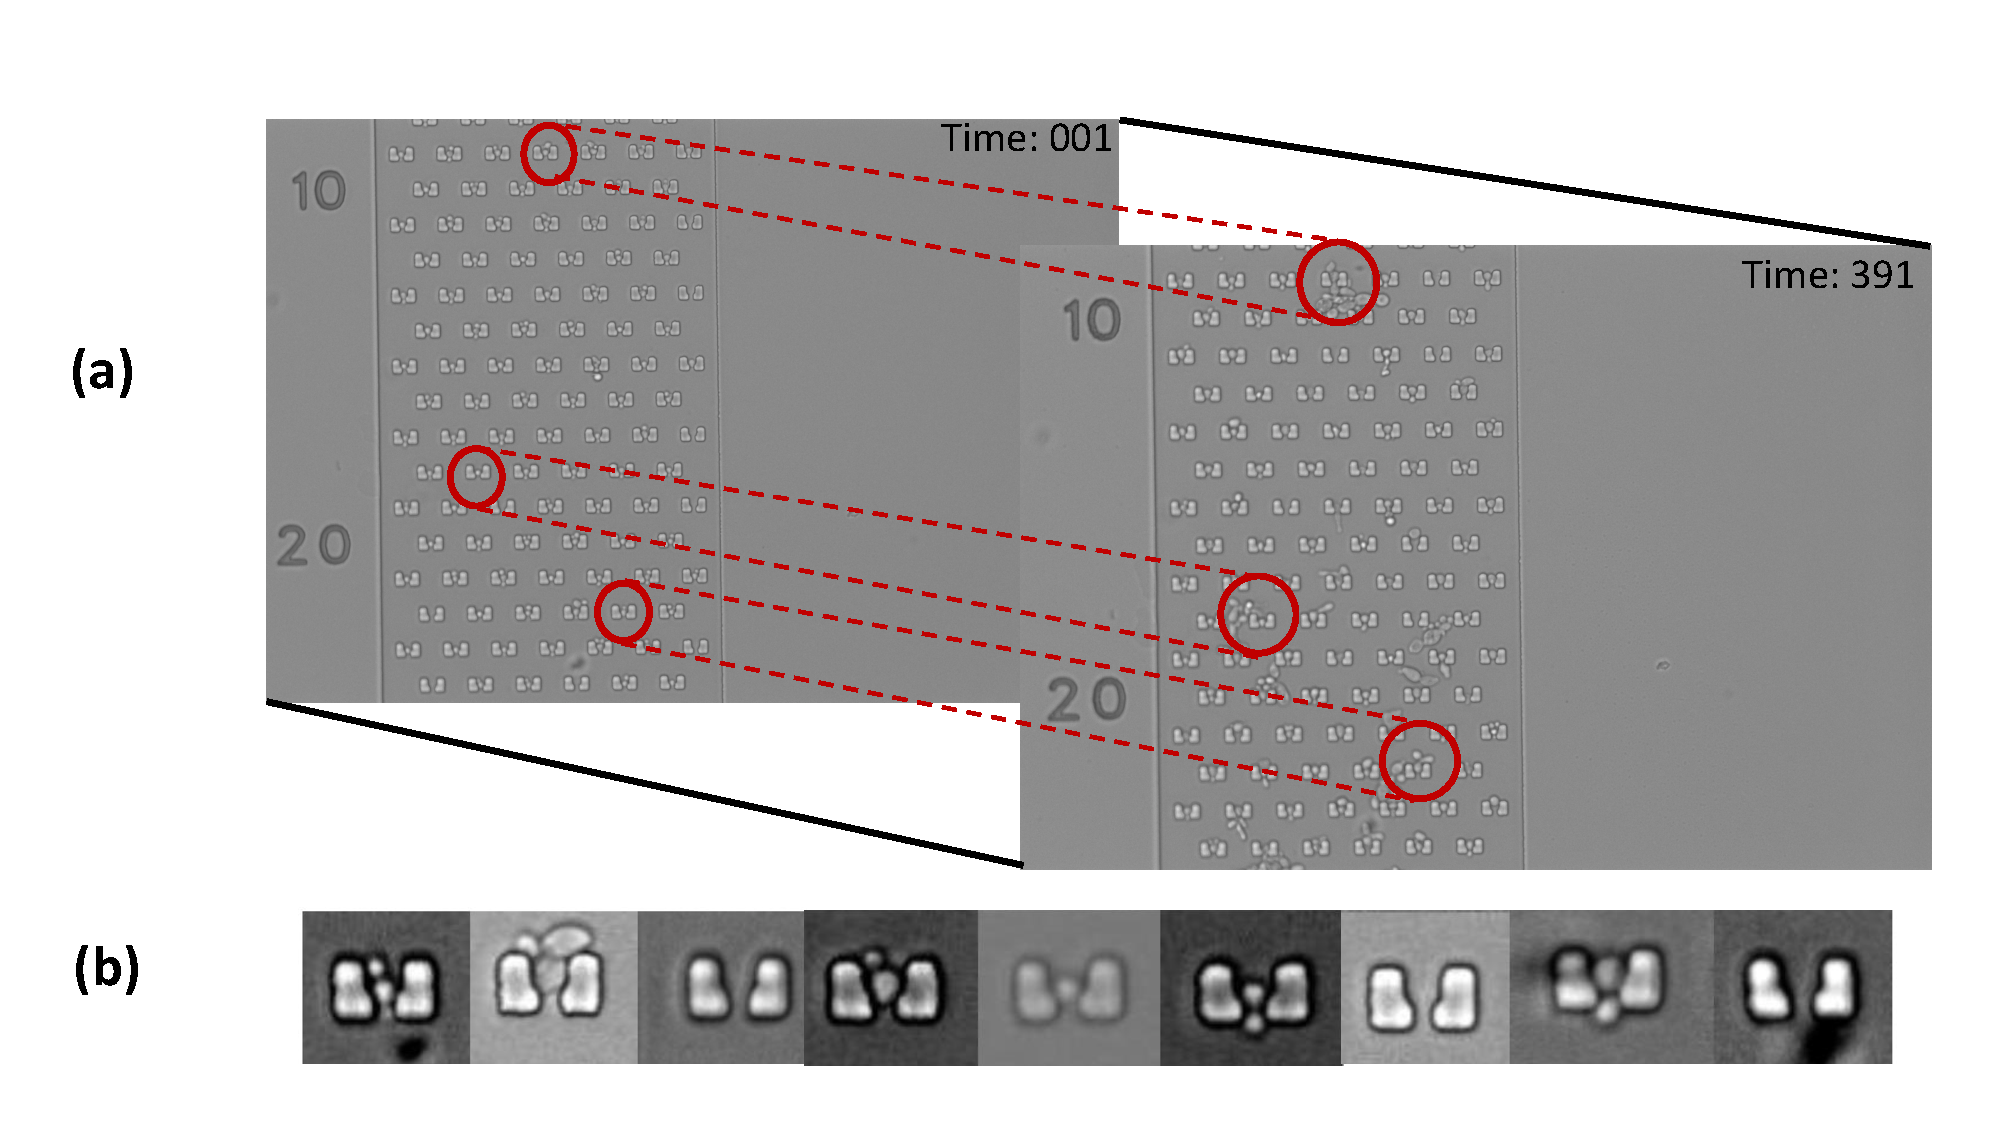
\includegraphics[width=1\textwidth,height=0.4\textheight]{dissertation/figures/plusone/S1_Fig_microfluidic.pdf}
\caption {Microfluidic Images.... }
\label{S1_Fig}
\end{figure} 

     %\include{back-matter/appendix-2}
     %\include{back-matter/appendix-3}

    %%%%%%%%%%%%%%%%%%%%%%%%%%%%%%%%%%%%%%%%%%%%%%%%%%%%%%%%%%%%%%%%%%%%%%%%%%%%%%%%%%%%%%%%%%%%%%%%%%%%%
    % A VITA IS REQUIRED
    %%%%%%%%%%%%%%%%%%%%%%%%%%%%%%%%%%%%%%%%%%%%%%%%%%%%%%%%%%%%%%%%%%%%%%%%%%%%%%%%%%%%%%%%%%%%%%%%%%%%%
    \makeVitaPage
\end{document}
